\exer{Bubble bobble}
\setcounter{numques}{0}

\begin{flushright}
\footnotesize{D'après Jean-Pierre Becirspahic.}
\end{flushright}
 On suppose disposer d’une fonction \texttt{circle(coords:list, r:float) -> None} qui trace à l’écran un cercle de centre 
 \texttt{coords=(x,y)} et de rayon \texttt{r}.
\ifprof\else
\begin{lstlisting}
import matplotlib.pyplot as plt
import numpy as np
def circle(coords:list, r:float) -> None :
    X, Y = [], []
    for t in range(101):
        X.append(coords[0]+r*np.cos(t*np.pi/50))
        Y.append(coords[1]+r*np.sin(t*np.pi/50))
    plt.plot(X, Y, 'b')
\end{lstlisting}
\fi

\question{Définir la fonction \texttt{bubble1(n:int, x:float, y:float, r:float) -> None} permettant de tracer la figure suivante.}
\ifprof
\begin{lstlisting}
def bubble1(n, x=0, y=0, r=8):
    circle([x, y], r)
    if n > 1:
        bubble1(n-1, x+3*r/2, y, r/2)
        bubble1(n-1, x, y-3*r/2, r/2)
\end{lstlisting}
\else
\begin{center}
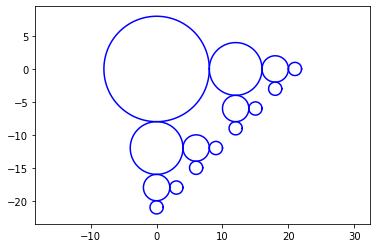
\includegraphics[width=.3\linewidth]{Fig1}
\end{center}
\fi
\question{Définir la fonction \texttt{bubble2(n:int, x:float, y:float, r:float, d:str) -> None} permettant de tracer la figure suivante.}
\ifprof
\begin{lstlisting}
def bubble2(n, x=0, y=0, r=8, d=''):
    circle([x, y], r)
    if n > 1:
        if d != 's':
            bubble2(n-1, x, y+3*r/2, r/2, 'n')
        if d != 'w':
            bubble2(n-1, x+3*r/2, y, r/2, 'e')
        if d != 'n':
            bubble2(n-1, x, y-3*r/2, r/2, 's')
        if d != 'e':
            bubble2(n-1, x-3*r/2, y, r/2, 'w')
\end{lstlisting}
\else
\begin{center}
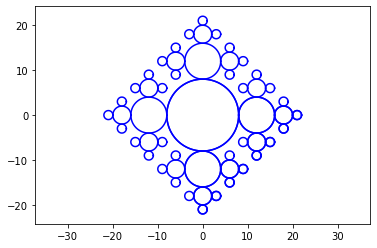
\includegraphics[width=.3\linewidth]{Fig2}
\end{center}
\fi